%=======================================================================
%
% ------------------------------------------------------------------------
% ------------------------------------------------------------------------
% abnTeX2: Modelo de Trabalho Academico  em conformidade com 
% ABNT NBR 14724:2011: Informacao e documentacao - Trabalhos academicos
% ------------------------------------------------------------------------
%Customização IFC
% ------------------------------------------------------------------------
% Autor:  Tiago Possato (tiago.possato@yahoo.com.br), baseado no modelo de Eliton Tiago (elitontiago@hotmail.com)
% Versão: 08 de Outubro de 2017.
% Codificação: UTF-8
% LaTeX:  abnTeX2
%
%=======================================================================

\documentclass[
	% -- opções da classe memoir --
	12pt,				% tamanho da fonte	
	oneside,          % não imprimir em verso e anverso, oposto do twoside 
	a4paper,			% tamanho do papel. 
	% -- opções da classe abntex2 --
	chapter=TITLE,		% títulos de capítulos convertidos em letras maiúsculas
	section=TITLE,		% títulos de seções convertidos em letras maiúsculas
	subsection=TITLE,	% títulos de subseções convertidos em letras maiúsculas
	%subsubsection=TITLE,% títulos de subsubseções convertidos em letras maiúsculas
	% -- opções do pacote babel --
	english,			% idioma adicional para hifenização
	brazil			% o último idioma é o principal do documento
	,sumario=tradicional,
	]{abntex2-IFC}


% ---
% Pacotes fundamentais 
% ---
\usepackage{cmap}				% Mapear caracteres especiais no PDF
\usepackage{times}			    % Usa a fonte Times
\usepackage[T1]{fontenc}		% Selecao de codigos de fonte.fontenc
\usepackage[utf8]{inputenc}		% Codificacao do documento (conversão automática dos acentos)
\usepackage{lastpage}			% Usado pela Ficha catalográfica
\usepackage{indentfirst}		% Indenta o primeiro parágrafo de cada seção.
\usepackage{color}				% Controle das cores
\usepackage{graphicx}			% Inclusão de gráficos
\usepackage{amsfonts}			% Símbolos
%----Ajuste no alinhamento das listas
\usepackage{enumitem}
\setitemize[0]{itemindent=0.4cm,itemsep=0pt}
\setenumerate[0]{itemindent=0.5cm,itemsep=0pt}
%------
% ---
% Pacotes de citações
% ---
\usepackage[brazilian,hyperpageref]{backref}	 					  % Paginas com as citações na bibl

\usepackage[a4paper]{geometry}
%Referência
\usepackage[alf, 	
			 		abnt-emphasize=bf,
				    abnt-url-package=none,
				    abnt-repeated-title-omit=yes,
				    abnt-full-initials=yes,                                        %yes nome por extenso, no apenas iniciais
					abnt-etal-list=3												%abreviar com mais de 3 autores
]{abntex2/abntex2cite}				 														    % Citações padrão ABNT
\usepackage{lipsum}							   								       % para geração de dummy text
\usepackage{multirow}
\usepackage{float}
\usepackage{setspace}
\usepackage{tabularx}

%\usepackage[none]{hyphenat}
%\captionsetup[table]{justification=raggedright}
% Configurações de aparência do PDF final
% alterando o aspecto da cor azul
\definecolor{blue}{RGB}{41,5,195}

% --- 
% Espaçamentos entre linhas e parágrafos 
% --- 
% O tamanho do parágrafo é dado por:
\setlength{\parindent}{2cm}
\linespread{1.5}

%Espaçamento depois dos títulos
\setlength{\afterchapskip}{\baselineskip}
% %\setlength{\afterchapskip}{\lineskip}

% Controle do espaçamento entre um parágrafo e outro:
\setlength{\parskip}{0cm}  % tente também \onelineskip

\hangcaption
\captionstyle[\raggedright]{}

%Estava mostrando nas referencias quais paginas estavam sendo referenciadas
\renewcommand{\backref}{}
\renewcommand*{\backrefalt}[4]{}

%Reduzir a fonte do caption
%\captionnamefont{\centering\ABNTEXfontereduzida}
%\captiontitlefont{\centering\ABNTEXfontereduzida}
%Ajuste nas listas de tabela, ilustrações e quadros
\setlength\cftbeforechapterskip{0pt}
% ---
% compila o indice
% ---
\makeindex
% ---

%----Include da capa é fora do documento 
% ---
% Informações de dados para CAPA e FOLHA DE ROSTO
% ---

\titulo{\uppercase{Título do trabalho}}
\autor{\uppercase{Nome do aluno}}
\local{Videira}
\data{Ano}
\orientador[Orientador:]{professor orientador}
\coorientador[Coorientador:]{professor coorientador}
\instituicao{ Ministério da Educação\\
        Secretaria de Educação Profissional e Tecnológica\\
        Instituto Federal Catarinense\\
        Câmpus Videira}
\tipotrabalho{Trabalho de Conclusão de Curso}
% O preambulo deve conter o tipo do trabalho, o objetivo, 
% o nome da instituição e a área de concentração
\preambulo{Trabalho de Conclusão de Curso apresentado ao
Curso de graduação em Ciência da Computação do
Instituto Federal Catarinense – Câmpus Videira para
obtenção do título de bacharel em Ciência da Computação.

Orientador: \imprimirorientador

Coorientador: \imprimircoorientador}
% ---


%---

\begin{document}
% Retira espaço extra obsoleto entre as frases.
\frenchspacing 

% ----------------------------------------------------------
% ELEMENTOS PRÉ-TEXTUAIS
% ----------------------------------------------------------

%--- CAPA ----
\imprimircapa

% --- FOLHA DE ROSTO
\imprimirfolhaderosto
% \imprimirfolhaderosto* (o * indica que haverá a ficha bibliográfica)

% Inserir FOLHA DE APROVAÇÃO
\begin{folhadeaprovacao}

  \begin{center}
  \vspace*{-1.2cm}
    \textbf{\large\imprimirautor}
    
    \vspace*{\fill}\vspace*{\fill}\vspace*{\fill}
    \parbox{15cm}{
        \OnehalfSpacing\centering\large\textbf{\imprimirtitulo}
    }
    \vspace*{\fill}\vspace*{\fill}
    
    \hspace{.45\textwidth}
    \begin{minipage}{.5\textwidth}
        Este Trabalho de Curso foi julgado
        adequado para a obtenção do título de
        Bacharel em Ciência da Computação e
        aprovado em sua forma final pelo curso de
        graduação em Ciência da Computação do Instituto Federal Catarinense
        – Campus Videira. 

    \end{minipage}%
    \vspace*{\fill}
   \end{center}
    \vspace{-1cm}
  \begin{center}
  	 Videira (SC), dia de mês de ano
  \end{center}
  

    %\vspace{-1cm}

  
   \assinatura{\begin{center}\vspace{-0.7cm}\imprimirorientador \\ 
   					   Instituto Federal Catarinense – Campus Videira
   					   \end{center}
   			  } 
    \assinatura{\begin{center}\vspace{-0.7cm}\imprimircoorientador \\ 
   					   Instituto Federal Catarinense – Campus Videira
   					   \end{center}
   			  } 
   			  
    \begin{center}
  	\textbf{ BANCA EXAMINADORA}
   \end{center}
   %\vspace{-1cm}
   \assinatura{\begin{center}\vspace{-0.7cm}FULANO\\ 
   					   Instituto Federal Catarinense – Campus Videira
   					     \end{center}
   }
    \assinatura{\begin{center}\vspace{-0.7cm}BELTRANO \\ 
   					    Instituto Federal Catarinense – Campus Videira
   					    \end{center}
    }
    

    \vspace*{1cm}
  
\end{folhadeaprovacao}

% Inserir FOLHA DE AUTORIZAÇÃO
% \begin{folhadeautorizacao}

  \begin{center}
  \vspace*{1 cm}
  \vspace{-2cm}
   \centering
\includegraphics[width=1.5cm]{brasaoRepublicaPeB.jpg}
   \vspace{-0.5 cm}
    {\large \SingleSpacing \imprimirinstituicao}
    \vspace{-0.5cm}
    \center{ \hrulefill}
    
     {\large \SingleSpacing \textbf{Autorização}}
    
    
    \vspace*{1 cm}
    
    \raggedleft{ Videira (SC), 19 de Novembro de 2016}
    \vspace*{0.5 cm}
    
   \end{center}
   


Eu, NOME SOBRENOME, regularmente matriculado na disciplina de Trabalho de Conclusão de Curso II - TC II do curso de Bacharel em Ciência da Computação, sob matrícula nº. XXXXXXX, pelo presente documento, autorizo o Instituto Federal Catarinense - IFC-Câmpus Videira, a utilizar o meu TC II intitulado "\imprimirtitulo", sob a orientação d Professor \imprimirorientador, para futuras informações e divulgações promovidas pelo Curso, e pelo Instituto, de forma institucional, em todo território nacional e internacional, sem fins comerciais, por qualquer meio de comunicação, tornando-o acessível a qualquer pessoa com interesse no trabalho.

A presente autorização substancia um consentimento de vontade e isenta de qualquer vício, feito de forma gratuita, e no gozo da minha capacidade civil, pelo que declaro nada me ser devido pelo curso de Ciência da Computação e pelo IFC-Câmpus Videira, ou seus representantes, em tempo algum, seja que título for, no que se refere, direta ou indiretamente, ao presente consentimento de uso da minha imagem e meu trabalho.

Declaro, ainda, que a utilização de meu nome e de meu trabalho, não constitui ofensa ou violação de meus direitos, nos termos do inciso X, do artigo 5o. da Constituição Federal.

Pelo presente também declaro ser de minha total responsabilidade o conteúdo de meu trabalho de conclusão de curso, descrito neste documento.

Os direitos e as obrigações aqui avençados transmitem-se aos meus herdeiros e sucessores.



  
   
   \vspace*{\fill}
   \vspace{-0.5 cm}
   
   \noindent Nome: \imprimirautor
   
   \vspace{0.25 cm}
   
   \noindent CPF: XXXXXXXXXXXXXX
   
   \vspace{0.25 cm}
   
   \noindent Assinatura: \hskip-3em\vtop{\vskip.05cm\hsize=5in \hrulefill}
   
   \vspace{0.5 cm}
   
    \begin{center}
    Rod. SC 135, KM 125 - Campo Experimental - CEP: 89560-000 - Videira - SC \\
    Fone: (49) 3533-4900 - http://www.ifc-videira.edu.br
    \end{center}

    \vspace*{1cm}
  
\end{folhadeautorizacao}

% DEDICATÓRIA
\begin{dedicatoria}
 \vspace*{\fill}
 \noindent
  \raggedleft
 \begin{minipage}{.54\textwidth}
    Dedico este trabalho ...
   \end{minipage}
\end{dedicatoria}


% AGRADECIMENTO
\begin{agradecimentos}

agradecimentos

\end{agradecimentos}

%EPÍGRAFE
\include{pretextuais/epigrafe}

% RESUMO
% resumo em português
\begin{resumo}
\noindent
 
Neste trabalho
 \vspace{0.2cm}   
Palavras-chave: palavra 1. palavra 2. palavra 3
 
\end{resumo}
 
% resumo em inglês
\begin{resumo}[Abstract]	
\begin{otherlanguage*}{english}
\noindent 
 
This is the abstract of this work.
 
\vspace{0.2cm}
Key-words: Word 1. Word 2. Word 3
\end{otherlanguage*}
\end{resumo}


% lista de ilustrações
\pdfbookmark[0]{\listfigurename}{lof}
\listoffigures*
\cleardoublepage
% ---

% lista de quadros
% --- 
%PRECISO VER COMO FAZER O CONTROLE DE QUANDO TIVER MENOS Q 10 VAI PARA LISTA DE ILUSTRAÇÕES
\pdfbookmark[0]{\listofquadrosname}{loq}
%\listofquadros*
%\cleardoublepage
% ---

% LISTA DE TABELAS
\pdfbookmark[0]{\listtablename}{lot}
%\listoftables*
%\cleardoublepage  %-- força proxima pagina

% ---
% inserir lista de abreviaturas e siglas
% ---
\begin{siglas}
  \item[SIGLA] descrição

\end{siglas}
% ---

% ---
% inserir lista de símbolos
% ---
%\begin{simbolos}
%  \item[$ \Gamma $] Descrever o que o símbolo representa em seu trabalho. Exemplo abaixo.
%  \item[$ \omega $] Frequência angular [rad/s].
%  \item[$ \zeta $] Coeficiente de amortecimento.

%\end{simbolos}
% ---

% SUMARIO
\pdfbookmark[0]{\contentsname}{toc}
\tableofcontents*
\cleardoublepage

% ------------------------------------------------------
% ELEMENTOS TEXTUAIS
% ------------------------------------------------------
\textual
% INTRODUÇÃO
\chapter{INTRODUÇÃO}

As orientações aqui apresentadas são baseadas em um conjunto de normas elaboradas pela ABNT. Além das normas técnicas a Biblioteca também elaborou  um guia para elaboração de trabalhos acadêmicos que está disponível na sua Homepage. < http://biblioteca.ifc.edu.br/normalizacao-de-trabalhos//>. 

\section{Objetivos}

\subsection{Objetivo Geral}
	
Descrição...

\subsection{Objetivos Específicos} 

Descrição...

% 
%--------- FIM INTRODUÇÃO------------
%

%Revisão
\chapter{DESENVOLVIMENTO}

\section{Exposição do Tema ou Matéria}

É a parte principal e mais extensa do trabalho detalhando o estudo ou a pesquisa realizada Deve apresentar a fundamentação teórica, a metodologia, os resultados e a discussão. Divide-se em seções e subseções conforme a NBR 6024. Quanto a sua estrutura, segue as recomendações da norma para preparação de trabalhos acadêmicos, a NBR 14724 de 2011. \cite{ABNT} 
Abaixo é apresentada a Figura \ref{fig:estrutura} onde se pode visualizar a estrutura geral do trabalho acadêmico.

\begin{figure}[htb]
	\caption{Estrutura geral}
    \centering
    {\parbox{16cm}{
	    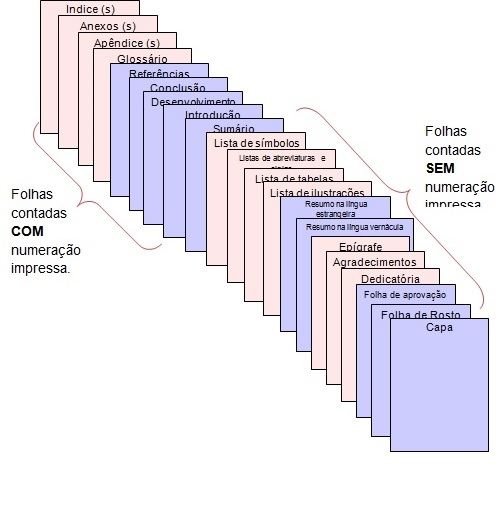
\includegraphics[width=16cm]{images/Fig1.jpg}
        \label{fig:estrutura}
		\fonte{Elaboração das Autoras, 2014}
    }}
\end{figure}


\section{Apresentação Gráfica do Trabalho Acadêmico}

A apresentação gráfica é a definição de tipo de fonte, margens, espaçamento, tipo de papel, etc.

\subsection{Formato (tipo de papel, tamanho da fonte, margens)}

A apresentação gráfica do TC deve seguir os seguintes requisitos:
a) utilizar papel branco ou reciclado, formato A4 (21,0 x 29,7 cm);
b) utilizar o anverso da folha para os elementos pré-textuais;
c) poderá ser utilizado o anverso e verso da folha para impressão dos elementos 
    textuais e pós-textuais;
c) digitar o texto na cor preta;
d) fonte tamanho 12 para o texto;
e) fonte tamanho 10 para citações longas, notas de rodapé, legendas e fontes 
    (identificação) das ilustrações e tabelas e paginação;
f) optar por fontes arredondadas (Times New Roman ou Arial);
g) adotar as margens:
    - para o anverso da folha:
       - superior de 3 cm, 
       - inferior de 2 cm,
       - esquerda de 3 cm,
       - direita de 2 cm,
     - para o verso:
        - superior de 3 cm, 
        - inferior de 2 cm,
        - esquerda de 2 cm,
       - direita de 3 cm,
h) primeira linha do parágrafo com recuo de 2 cm a partir da margem esquerda;
          i) citação longa (com mais de três linhas) com recuo de 4 cm a partir da margem
    esquerda;
j) nota de rodapé digitada dentro das margens indicadas, devendo ficar separada do 
   texto por um traço de 5 cm a partir da margem esquerda.

\subsection{Espaçamento}

O espaçamento que você deve adotar na formatação é:
a) espaço 1,5  - todo o texto,
          b) um espaço de 1,5;
     - separa o texto da citação longa,
     - separa cada título das seções e subseções do texto que os precedem e que os 
       sucedem,
c) espaço simples para;
    - citações longas,
    - notas de rodapé,
    - referências,
    - legenda e fonte das ilustrações e tabelas,
    - natureza do trabalho.
e) um espaço simples -  entre uma referência e outra, na lista de referências ao final do trabalho.

\subsection{Indicativo de seção e numeração progressiva}

Seção é a divisão do TC, aplicada somente aos elementos textuais e visa expor numa sequência lógica o relacionamento da matéria e a permitir a sua localização. De acordo com a NBR 6024 as seções também podem ser subdividas em subseções.
A seção primária é a principal divisão do texto do TC, que sempre deverá ser grafada em números inteiros a partir do 1, alinhados à esquerda por um espaço de caractere e iniciar em página distinta e ímpar (anverso). As demais são chamadas de subseções e/ou seções secundária, terciária, quaternária e quinária. Se for necessário enumerar os diversos assuntos de uma seção que não possua título, esta deve ser subdividida em alíneas. As alíneas são ordenadas alfabeticamente e terminam em ponto e vírgula, exceto a última que termina em ponto. Todas as seções devem conter um texto relacionado a elas (FIGURA \ref{fig:secoes}) .
Exemplo sugerido pelo IFC:
1 SEÇÃO PRIMÁRIA (maiúsculas em negrito)
1.1 SEÇÃO SECUNDÁRIA (maiúsculas)
1.1.1 Seção terciária (em negrito com primeira letra maiúscula)
1.1.1.1 Seção quaternária (primeira letra maiúscula)
1.1.1.1.1 Seção quinária (em itálico com primeira letra maiúscula)
a) alínea (primeira letra minúscula);
b) alínea;
    - subalínea.
c) alínea.
2 SEÇÃO PRIMÁRIA 
2.1 SEÇÃO SECUNDÁRIA 
2.1.1 Seção terciária 
.
.
.
\begin{figure}[htb]
	\caption{Seções}
    \centering
    {\parbox{16cm}{
		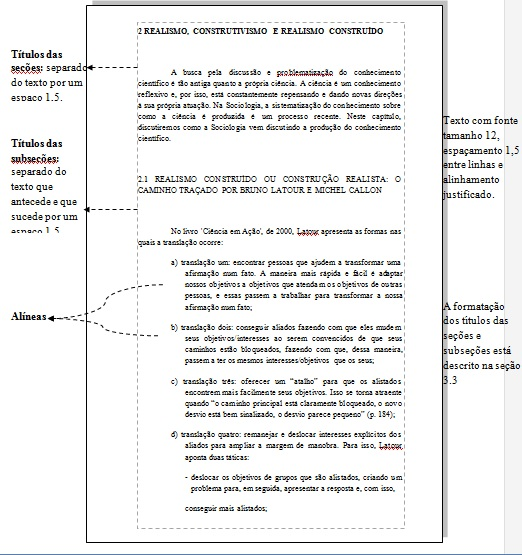
\includegraphics[scale=1.1]{images/Fig2.jpg}
	    \label{fig:secoes}
	    \hspace{0.0cm}{Fonte: Elaboração das Autoras, 2014}
    }}
\end{figure}


\subsection{Paginação}

Para o TC, as páginas pré-textuais devem ser contadas, mas não numeradas. A contagem será a partir da folha de rosto. A numeração deve configurar a partir da primeira folha textual em algarismos arábicos e sendo sequencial até o final do trabalho. 
A paginação da(s) referência(s), do(s) anexo(s) e do(s) apêndice(s) deve ser numerada sequencialmente no TC. As páginas que não permitem a inclusão de números também são contadas (mapas, documentos, ilustrações, etc.).
O número da página deve aparecer no canto superior direito da folha, a 2 cm da borda superior, ficando o último algarismo a 2 cm da borda direita da folha.
Para trabalhos com mais de um volume, a numeração sequencial das folhas deve ser mantida. Se o trabalho contiver apêndice e anexo, a numeração das páginas deve dar sequência ao texto principal.

\subsection{Lombada}

A lombada é um elemento opcional para o TC e na sua estrutura, deve conter os seguintes elementos: 
a)	nome(s) do(s) autores, quando houver;
b)	título;
c)	identificação do volume, fascículo e data, se houver.
Todos os elementos que compõem a lombada devem ser centralizados em suas áreas, com fonte tamanho 12, espaçamento simples e todas as letras maiúsculas (FIGURA \ref{fig:lombada}).

\begin{figure}[h]
	\caption{Lombada}
    \centering
    {\parbox{16cm}{
		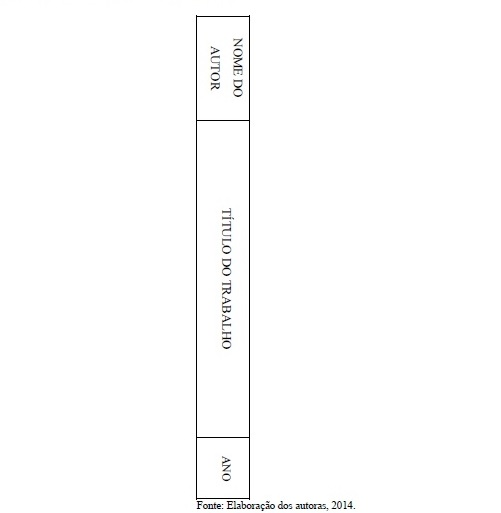
\includegraphics[scale=1.1]{images/Fig3.jpg}
	    \label{fig:lombada}
	    \hspace{5.7cm}{Fonte: Elaboração das Autoras, 2014}
    }}
\end{figure}

% 
%--------- FIM DESENVOLVIMENTO------------
%

%CONCLUSÃO
\chapter{CONCLUSÃO}

As conclusões devem responder às questões da pesquisa, em relação aos objetivos e hipóteses. Devem ser breves podendo apresentar recomendações e sugestões para trabalhos futuros.  

% ----------------------------------------------------------
% ELEMENTOS PÓS-TEXTUAIS
% ----------------------------------------------------------
\postextual

% ----------------------------------------------------------
% Referências bibliográficas
% ----------------------------------------------------------

\bibliography{referencias}

%Apêndices
% \begin{apendicesenv}

\chapter{Título do Apêndice A}

Arquivos confeccionados pelo autor do trabalho e que não se encaixam no texto.

 Ex: Deduções matemáticas, dimensionamentos extensos e algoritmos.

\end{apendicesenv}

%Anexos
% \begin{anexosenv}
\chapter{Título do Anexo A}
\label{anexoA}

Arquivos não confeccionados pelo autor do trabalho.


\end{anexosenv}

%---------------------------------------------------------------------
% INDICE REMISSIVO
%---------------------------------------------------------------------
% \printindex
\end{document}